\documentclass{article}
\usepackage{fullpage} %small margins etc.
%\usepackage{algorithmic} %pseudocode
%\usepackage{algorithm} %pseudocode as whole procedures
%\usepackage{program} %more sophisticated pseudocode
%\usepackage{amssymb} % mathematical symbols (if you use program, comment this)
\usepackage{pseudocode}
\usepackage{url} %url addresses
\usepackage{multirow}
%\usepackage{booktabs}
%\usepackage{color}
\usepackage{graphicx} %images
\usepackage{float} %for proper placement of floating figures

\providecommand{\e}[1]{\ensuremath{\times 10^{#1}}}

\newcommand{\comment}[1]{}

\begin{document}

\title{Halley's Method and Jarratt's Method implementations}
\date{May 30, 2011}
\author{Bysiek Mateusz, Witan Maciej (Computer Science A/R)}
\maketitle

\section{Task}

Write a computer program to implement the Halley and the Jarratt's methods for
finding a root of the complex polynomial

\[ p(x) = \sum_{k=0}^{n}{a_k x^k}  \]

Use Horner's scheme. Compare the results.

\section{Theoretical introduction}

\subsection{Basics of approximation}

The approximation of values of functions is a very important topic in mathematics. This is the area
where beautiful mathematical formulas meet with the real problems of engineering and the financial
world. Among the most characteristic problems within the field of approximation, there is a problem
of root finding.

One of the solutions to this problem is iteration. In this approach, you do not go directly to the
final solution, but rather get close to it in your first step, and then get closer and closer in
each subsequent step, until you reach your desired precision. If $x_k$ is the k-th step of
iteration, then:

\[ x_k \stackrel{k \rightarrow \infty}{\longrightarrow} \alpha \Longrightarrow f(\alpha) = 0 \]

For such approach, one needs an initial guess $x_0$. Usually, one should form a vector of initial
guesses in case of $x \in R$ or a matrix in case of $x \in C$. The tollerable error value should
also be chosen. Then, starting from every field, one launches iteration using the chosen method. In
vast majority of cases, if after around 20 iterations the method will not converge, it means that it
diverges and will not find a proper root for this guess at all.

To sum up, no method is 100\% reliable, and some are better in one types of functions, whereas
other are better in approximation of other types of functions.

Our task was to find roots of polynomials of higher orders. There are many methods for those
wishing to find those roots, some of them are fast, but not precise. Other are more precise, but
also slower, and they may require very favorable initial conditions, to end successfully. The
question arises: how fast does your iterative method converge?

To differentiate all the methods, the idea of rate of convergence was born. The higher that rate
is, the faster the given method converges. Almost all widely used approximation methods work well
not only in the field of real numbers, but also with functions of complex variables (polynomials of
complex coefficients and/or complex roots). The exception here is the Bisection Method, although it
is not the role of this paper to describe it in detail.

\subsection{Newton's Method}

We will, however, describe the two methods that we have implemented. Both of the methods we are
analysing in this paper have been derived from the Newton's Method. Thus, the ``parent'' looks like
this:

\begin{center}
\[ x_1 = x_0 - \frac{f(x_0)}{f'(x_0)} \]
(\ldots)
\[ x_{n+1} = x_n - \frac{f(x_n)}{f'(x_n)} \]
\end{center}

In above: $x_0$ is the initial guess, $x_n$ is the solution after the $n^{th}$ iteration. The
Newton's method has rate of convergence equal to $2$. In case of our task, both Halley's and
Jarratt's methods have rate of convergence equal to $3$, so they converge faster. But, do they
behave in the same way?

\subsection{Halley's Method in detail}

\subsubsection{Mathematical properties}

The method is used for functions of one real variable with a continuous second derivative. It is
named after its inventor Edmond Halley, who also discovered Halley's Comet. As mentioned earlier,
the rate of convergence to the root is cubic. That kind of rate means quite quick convergence.
Formula of this method is as follows:

\[ x_{n+1} = x_n - \frac{2 f(x_n) f'(x_n)}{2 [f'(x_n)]^2 - f(x_n)f''(x_n)} \]

\subsubsection{Pseudocode}

For the purpose of being clearer to the reader, as well as better relation to our actual script, we
have divided the pseudocode into two parts.

Single step of the approximation is called halleyStep. This function takes the polynomial $p$ and
current approximation of the root $x0$. It returns the corrected value $x$ and the tollerance $tol$.

\begin{pseudocode}{halleyStep}{p, x_0}
	x \gets x_0 \\
	n \gets length(p)-1 \\
	a \gets n:-1:1 \\
	q \gets a.*p(1:n) \\
	b \gets (n-1):-1:1 \\
	u \gets b.*q(1:n-1) \\
	corr \gets (2 \times polyval(p,x) \times polyval(q,x) ) / (2 \times polyval(q,x)^2 - polyval(p,x)
	\times polyval(u,xi)) \\
	x \gets x - corr \\
	tol \gets corr \\
	\RETURN{x, tol}
\end{pseudocode}

Main algorithm of the whole Halley's method uses the above-described code. The function
takes polynomial $p$, the initial guess $x0$, tollerance $tol$, and maximum number of iterations
$maxIter$. It returns the final solution $x$ and number of iterations $l$. If the function returns
$l = maxIter$, it means that most probably the final solution is wrong, and therefore, our initial
guess was too far from the correct solution.

\begin{pseudocode}{halleyMethod}{p, x_0, tol, maxIter}
	\IF x_0 = 0 \THEN
		x_0 \gets tol \\
	x \gets x_0 \\
	l \gets 0 \\
	flag\gets 0 \\
	\WHILE flag = 0 \DO
	\BEGIN
		\left[ x,corr \right] = halleyStep(p, x) \\
		\IF norm(corr) \leq tol \THEN
			flag \gets 1 \\
		\IF l > maxIter \THEN
			flag \gets 1 \\
		l \gets l+1 \\
	\END \\
	\RETURN{x, l}
\end{pseudocode}

\subsection{Jarratt's Method in detail}

\subsubsection{Mathematical properties}

Jarrat's Method was introduced in 1966. Interestingly, it has rate of convergence equal to 3, the
same as Halley's, but does not require taking second derivative of the given function. Therefore, it
can be used on functions that do not have continous second derivative, but more or less keeps the
convergence rate. The formula is as follows:

\[ x_{n+1} = x_n - \frac{f(x_n)}{f'( x_n-\frac{1}{2}f(x_n)/f'(x_n) )} \]

\subsubsection{Pseudocode}

The procedure of finding the root is similar, however, the core of the algorithm is different.
Still, both functions take the same arguments, and are expected to yield results in exact same
format.

\begin{pseudocode}{jarrattStep}{p, x_0}
	x \gets x_0 \\
	n \gets length(p)-1 \\
	a \gets n:-1:1 \\
	q \gets a.*p(1:n) \\
	t \gets x - 0.5 \times polyval(p,x) / polyval(q,x) \\
	corr \gets polyval(p,x) / polyval(q,t) \\
	x \gets x - corr \\
	tol \gets corr \\
	\RETURN{x, tol}
\end{pseudocode}

\begin{pseudocode}{jarrattMethod}{p, x_0, tol, maxIter}
	\IF x_0 = 0 \THEN
		x_0 \gets tol \\
	x \gets x_0 \\
	l \gets 0 \\
	flag\gets 0 \\
	\WHILE flag = 0 \DO
	\BEGIN
		\left[ x,corr \right] = jarrattStep(p, x) \\
		\IF norm(corr) \leq tol \THEN
			flag \gets 1 \\
		\IF l > maxIter \THEN
			flag \gets 1 \\
		l \gets l+1 \\
	\END \\
	\RETURN{x, l}
\end{pseudocode}

\section{Implementation}

To implement the above-mentioned methods, we have chosen MATLAB environment. The backbone of both
algorithms is very similar, therefore implementations of both methods look very alike.

\subsection{Halley's Method}

Two files: $halleyStep.m$ and $halleyMethod.m$, contain the implementations of Algorithms 2.1 and
2.2 from this document.

\subsection{Jarratt's Method}

The second method is also implemented in two files, each of which has very similar design to the
files comprising the Halley's Method. File $jarrattStep.m$ contains Algorithm 2.3 and file
$jarrattMethod.m$ contains Algorithm 2.4.

\section{Examples}

Using MATLAB's built in tool to draw color maps, we have created four examples with two color maps
for each. Scale on the right of every graph shows the number of iterations needed to reach
convergence. The maximum number of steps (after which the algorithm ends regardless whether it
was converging or not) was set to 25.

The file $examples.m$ contains four example polynomials, which we have described in ``Examples''
section of this document, below. The files $halleyColor.m$ and $jarrattColor.m$ contain example
usage of the methods, together with color maps.

In the examples, we use random number generator, but to get results that may be repeated by the
reader, we do this:

\[rand('state',0)\]

\subsection{First polynomial}
As a warm-up, very easy function, generated with the formula: $p_1 = poly(rand(1,9) + i*rand(1,9))$

\[ p_1(x) \approx 1x^9 + (-5.2-6i)x^8 + (-3.7+27.8i)x^7 + (48.9-32.3i)x^6 + (-76.6-21.3i)x^5 +\]
\[ + (31.2+65.7i)x^4 + (18-41.2i)x^3 + (-17.2+5.4i)x^2 + (3.7+2.2i)x^1 + (-0.1-0.5i) \]

Both Halley's and Jarratt's Methods dealt with this problem quite quickly. Halley's Method (Figure
1) was slightly faster, but as one can see on attached graphs, both of the methods had the same
ares of faster and slower convergence.

\begin{figure}[H]
	\begin{minipage}[b]{0.48\linewidth}
		\centering
		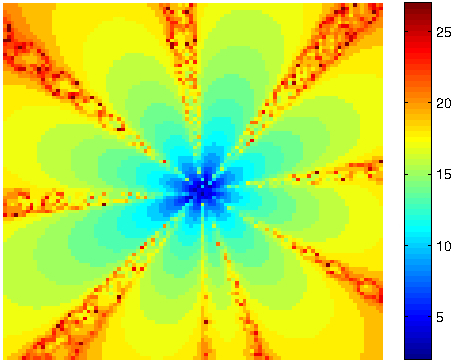
\includegraphics[scale=0.68]{example1halley.jpg}
		\caption{$1^{st}$ example, Halley's Method}
		\label{fig:figure1}
	\end{minipage}
	\hspace{0.5cm}
	\begin{minipage}[b]{0.48\linewidth}
		\centering
		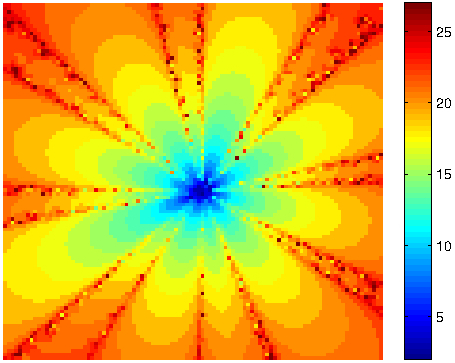
\includegraphics[scale=0.68]{example1jarratt.jpg}
		\caption{$1^{st}$ example, Jarratt's Method}
		\label{fig:figure2}
	\end{minipage}
\end{figure}

\subsection{Second example}
The second polynomial looks as follows: $p_2 = poly([1,1,1,1,i,i,i,-i,1+i,1+i,1+i])$

\[ p_2(x) = (x-1)^4(x-i)^3(x-1-i)^3(x+i) \]

In this example the multiplicity of the polynomial's roots plays the most signifficant role. In case
of multiple roots, the initial guess has to be close to the actual solution, otherwise both methods
fail to converge. In case of simple roots, both methods converge in just a few iterations, and
Halley again requires fewer.

\begin{figure}[H]
	\begin{minipage}[b]{0.48\linewidth}
		\centering
		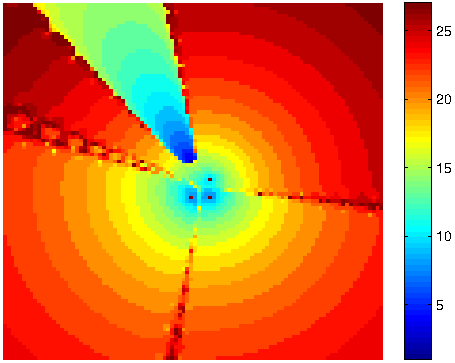
\includegraphics[scale=0.68]{example2halley.jpg}
		\caption{$2^{nd}$ example, Halley's Method}
		\label{fig:figure3}
	\end{minipage}
	\hspace{0.5cm}
	\begin{minipage}[b]{0.48\linewidth}
		\centering
		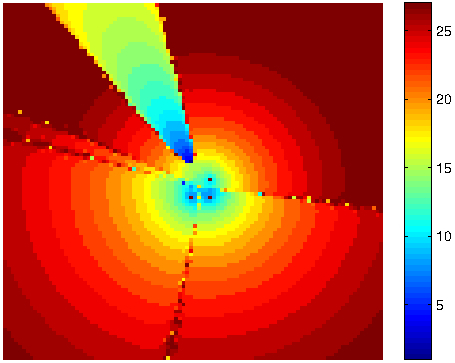
\includegraphics[scale=0.68]{example2jarratt.jpg}
		\caption{$2^{nd}$ example, Jarratt's Method}
		\label{fig:figure4}
	\end{minipage}
\end{figure}

\subsection{Third polynomial}
The third example, based on Wilkinson's polynomial: $w_3 = poly(1 : 1 : 100)$

\[w_3(x)=(x-1)(x-2)(x-3) \ldots (x-98)(x-99)(x-100)\]

The Wilkinson's polynomial itself is a specific polynomial which was used by James H. Wilkinson in
1963 to illustrate a difficulty when finding the root of a polynomial: the location of the roots can be
very sensitive to perturbations in the coefficients of the polynomial. It was designed as a
polynomial having an arbitrary number of integer roots: $1, 2, 3, \ldots ,n-1, n$. In our case,
there are 100 roots. The main characteristic of this function is that it has very high coefficients
of the $x$ terms of higher order. This causes it to be very ill conditioned.

Halley's Method converges only when the intitial guess is near to the correct answer. In case of any
signifficant distance between the initial guess and any root, the method diverges. The reason is
that this polynomial has very large values between the roots, since the floating point numbers
lose all of their precision when operating on numbers with large integer part.

Jarratt's Method performs better, but still the so-called ``Willkinson's monster'' gives it the hard
time.

\begin{figure}[H]
	\begin{minipage}[b]{0.48\linewidth}
		\centering
		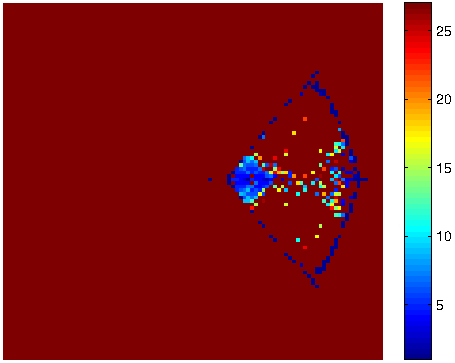
\includegraphics[scale=0.68]{example3halley.jpg}
		\caption{$3^{rd}$ example, Halley's Method.}
		\label{fig:figure5}
	\end{minipage}
	\hspace{0.5cm}
	\begin{minipage}[b]{0.48\linewidth}
		\centering
		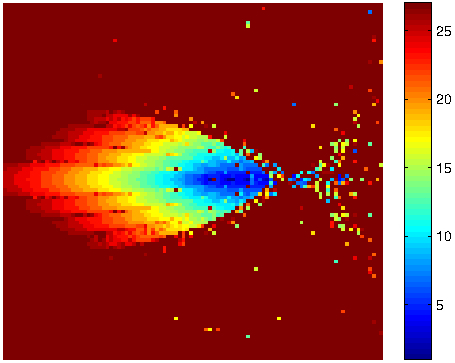
\includegraphics[scale=0.68]{example3jarratt.jpg}
		\caption{$3^{rd}$ example, Jarratt's Method.}
		\label{fig:figure6}
	\end{minipage}
\end{figure}

\subsection{Fourth polynomial}
The fourth and the last example included in our work is the polynomial which is very difficult to
approximate for both methods. The formula is as follows:
\[w_4 = poly(ones(1,10) + i*(1e-10) * rand(1,10)) \]

The roots of this polynomial are very close to each other, and because of that, the initial guess
already has to be close to the exact solution, for any of those two methods to converge. Jattatt's
Mehtod performs good when starting in close proximity of the target. On the other hand, for Halley's
Method, the area on which the correct answers are found is wider, but the total number of initial
guesses that ended in convergence is lower.

\begin{figure}[H]
	\begin{minipage}[b]{0.48\linewidth}
		\centering
		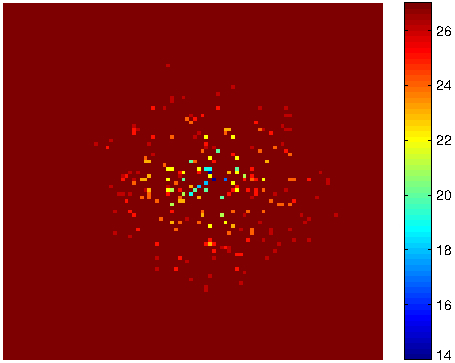
\includegraphics[scale=0.68]{example4halley.jpg}
		\caption{$4^{th}$ example, Halley's Method.}
		\label{fig:figure7}
	\end{minipage}
	\hspace{0.5cm}
	\begin{minipage}[b]{0.48\linewidth}
		\centering
		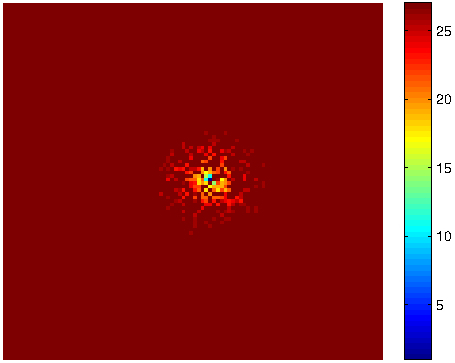
\includegraphics[scale=0.68]{example4jarratt.jpg}
		\caption{$4^{th}$ example, Jarratt's Method.}
		\label{fig:figure8}
	\end{minipage}
\end{figure}

\section{Comparison of numerical results}

All tables in this section use the following shortcuts:
\begin{itemize}
  \item result: solution provided by the method, after it ended 
  \item steps: number of steps for a given method until reaching tolerable solution
\end{itemize}

The tolerance for our examples was set to $0.001$.

\subsection{More details for example polynomial no.1}
In the set of roots of the polynomial mentioned earlier, there are such numbers:
\[0.60684258\underline{35417866} +0.79193703\underline{74270354}i\]
\[0.8214071642\underline{952533} +0.9169044399\underline{134076}i\]

Underlined digits in the above mean that error was at most that big, and underlined digits in table
below emphasise size of the error of calculations.

\begin{tabular}{rrrrr}
\multicolumn{2}{c}{} & \multicolumn{2}{c}{} \\
method & initial guess & result & steps \\
\hline
Halley & \multirow{2}{*}{1 + 5i}
& 0.6068425835\underline{608280} + 0.79193703742\underline{15257}i & 15 \\
Jarratt &
& 0.60684258\underline{28269729} + 0.79193703\underline{88755362}i & 16 \\

Halley & \multirow{2}{*}{1.5 + 5i}
& 0.6068425835\underline{630573} + 0.791937037\underline{3940863}i & 15 \\
Jarratt &
& 0.60684258\underline{45474732} + 0.79193703\underline{59690249}i & 16 \\

Halley & \multirow{2}{*}{2 + 5i}
& 0.6068425835\underline{512001} + 0.7919370374\underline{113323}i & 17 \\
Jarratt &
& 0.6068425835\underline{571063} + 0.79193703742\underline{09735}i & 18 \\

Halley & \multirow{2}{*}{2.5 + 5i}
& 0.8214071642\underline{775634} + 0.9169044399\underline{240325}i & 15 \\
Jarratt &
& 0.8214071642\underline{853524} + 0.91690443991\underline{83010}i & 18 \\

Halley & \multirow{2}{*}{3 + 5i}
& 0.8214071642\underline{860094} + 0.91690443991\underline{81225}i & 15 \\
Jarratt &
& 0.8214071642\underline{793698} + 0.91690443991\underline{67766}i & 17 \\
\end{tabular}
\vspace{10pt}

In this case (case of an ordinary polynomial) Halley's Method converges faster in all provided
examples. Both algorithms present similar precision, in some cases Halley converged closer, in other
it was Jarratt.

%\subsection{New example}

%(\ldots)

\section{Conclusion}

After running some more examples, we have reached the conclusion that, as expected because of common
ancestor (Newton's Method), both Halley's and Jarratt's methods perform in similar fashion, and they
in general have many common strong-points and weak-points. Halley's Method performs slightly better
in general, as the number of steps in most initial guesses is smaller when compared to the number of
steps that Jarratt's Method needed. Jarratt's Method performs slightly better when dealing with
functions that have large values and change rapidly, because the impact on the method that use only
the $1^{st}$ derivative of such function is smaller, when compared to the impact on the method that
derives twice.

To sum up, our observations confirm that both methods should have the same rate of convergence, and
that they both are improved versions of Newton's Method. We hope that this paper will help the
reader with making a choice, which method of approximation to use in his or her real-life problem :)

\section{Sources}

\begin{itemize}

	\item J. M. McNamee - \emph{Numerical methods for roots of polynomials, Part 1}, Elsevier B.V.,
	Amsterdam, First Edition, 2007
	
	\item \url{http://en.wikipedia.org/wiki/Newton's_method}
	
	\item \url{http://en.wikipedia.org/wiki/Halley's_method}
	
	\item \url{http://en.wikipedia.org/wiki/Wilkinson's_polynomial}

\end{itemize}

\section{High quality color maps}
On the following pages there are high resolution images representing convergence for examples from
Section 4. They somehow better illustrate the arguments made earlier in this document.

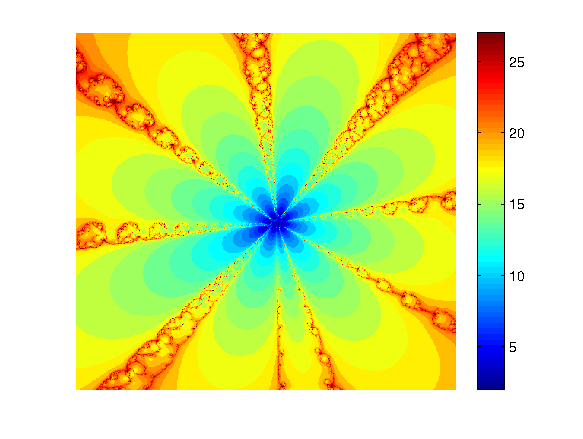
\includegraphics[scale=0.95]{example1halleyHigh.jpg}

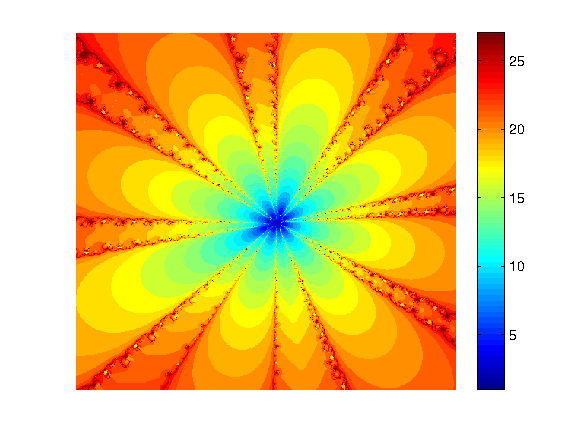
\includegraphics[scale=0.95]{example1jarrattHigh.jpg}

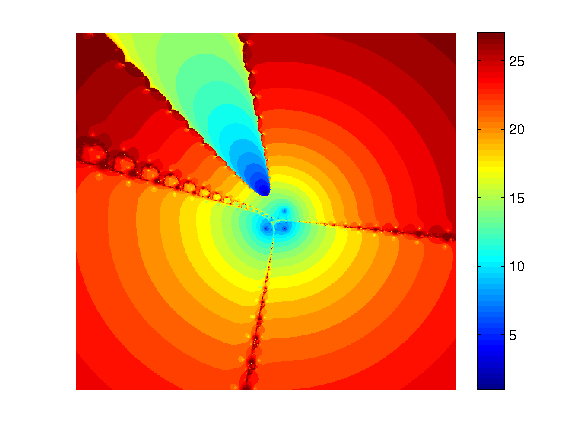
\includegraphics[scale=0.95]{example2halleyHigh.jpg}

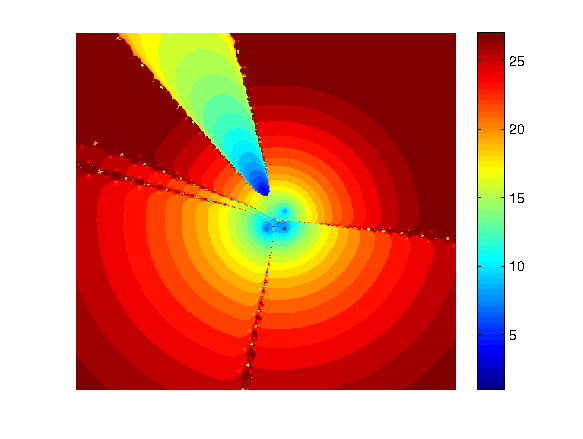
\includegraphics[scale=0.95]{example2jarrattHigh.jpg}

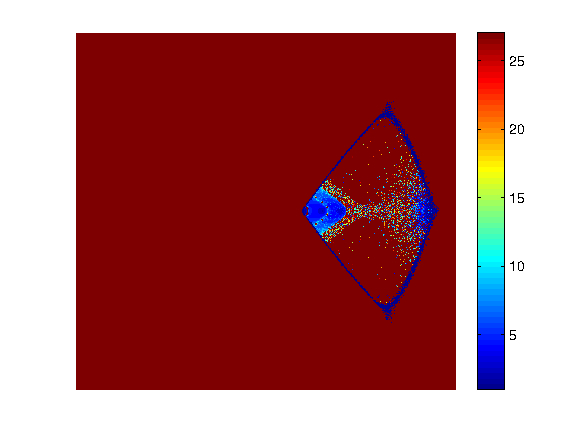
\includegraphics[scale=0.95]{example3halleyHigh.jpg}

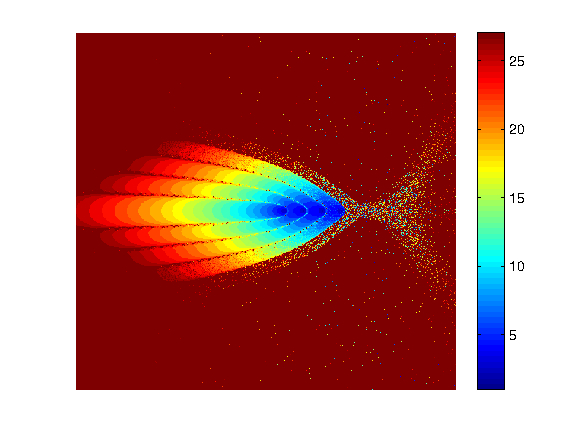
\includegraphics[scale=0.95]{example3jarrattHigh.jpg}

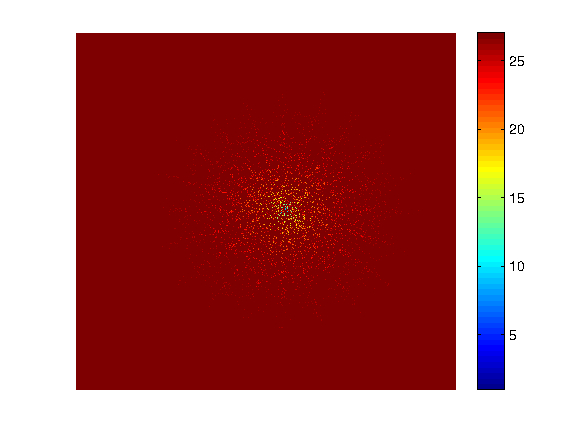
\includegraphics[scale=0.95]{example4halleyHigh.jpg}

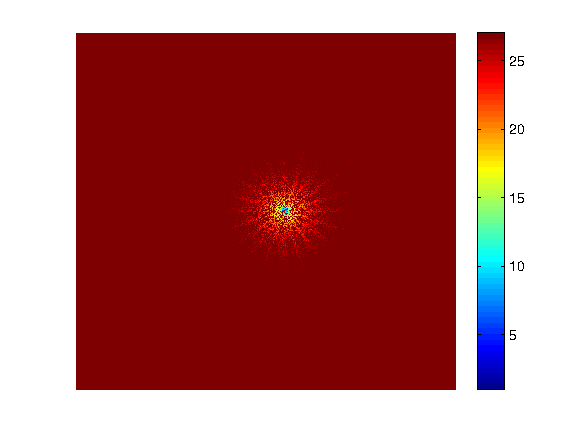
\includegraphics[scale=0.95]{example4jarrattHigh.jpg}

\end{document}
